\section{导数}\label{012}

\begin{tcolorbox}[size=fbox, breakable, enhanced jigsaw, title={导数 (derivative)}]

初中阶段常有求二次函数切线的题目,
利用初中知识求切线的表达式往往过程冗长, 事实上, \textbf{微积分}
(calculus) 会大大简化这个过程. 微积分, 如其名所示, 分为\textbf{微分}
(differentiation) 和\textbf{积分 }(integration).

在这里我们姑且先用经典的角度来了解微积分. \textbf{微分} (differential)
可以不严谨的理解为\textbf{无穷小量} (infinitesimal),
这是一些物理教材中更常见的表述, 例如某函数 $y=f(x)$,
它的一个有限的变化通常记作 $\Delta y$, 这个小三角念作``delta'',
在很多场景下表示变化, 而一个无穷小量的变化便记作 $\mathrm{d}y$.
任何实数都比无穷小量大, 就像无穷大 $\infty$ 大于任何实数\footnote{\ref{007}\nameref{007}中有提到过``浮点数'', 例如一个有理数 a,
它不会被以分数的形式记录, 而是记录其小数形式并精确到某一位,
那么第一个非零位数低于这一位的数字 b, 它对于 a 来说在计算机数值上看来,
便等效于无穷小量. 在 MATLAB 中, 给定一个实数 a, 利用函数 eps(), eps(a)
便会输出对于 a 来说的``无穷小量''.}.

另有一个非常类似的概念叫做\textbf{导数}, 导数可以理解为函数的变化率.
考虑某函数 $y=f(x)$ 在一个很小但是有限的一个定义域区间 $[a,b]$,
有自变量的变化为 $\Delta x=b-a$, 函数值的变化为
$\Delta y= f(b)-f(a)$, 于是在此区间内``平均''变化率是

$\frac{\Delta y}{\Delta x}=\frac{f(b)-f(a)}{b-a}.$

若是希望得到 $x=a$ 处的瞬时变化率, 我们令 $h:=b-a$, 直觉上应该是
$\lim_{h\rightarrow0}[f(a+h)-f(a)]/h$, 这便是函数 $f(x)$ 在 $x=a$
处的变化率, 或 $f(x)$ 在 $x=a$ 处的导数. 推广到任意位置 $x$, 遂有:

\begin{tcolorbox}[size=fbox, breakable, enhanced jigsaw, title={定义}]
函数 $f(x)$ 的导(函)数\footnote{取某个特定的点 $x=x\_0$,
  得到的导数是一个具体数值, 便叫它导数; 若不将 $x$ 锚定到一个特定的值,
  导数便依旧是一个含 $x$ 的函数, 便叫它导函数. 下文不再区分. 类似的,
  后文再出现的微分, 导数和无穷小量也不再严格区分.}为

$\lim_{h\rightarrow0}\frac{f(x+h)-f(x)}{h}.$
\end{tcolorbox}

很多数学教材会这么标记导数

$\boxed{f'(x)=\lim_{h\rightarrow0}\frac{f(x+h)-f(x)}{h}}.$

\begin{tcolorbox}[size=fbox, breakable, enhanced jigsaw, sidebyside]
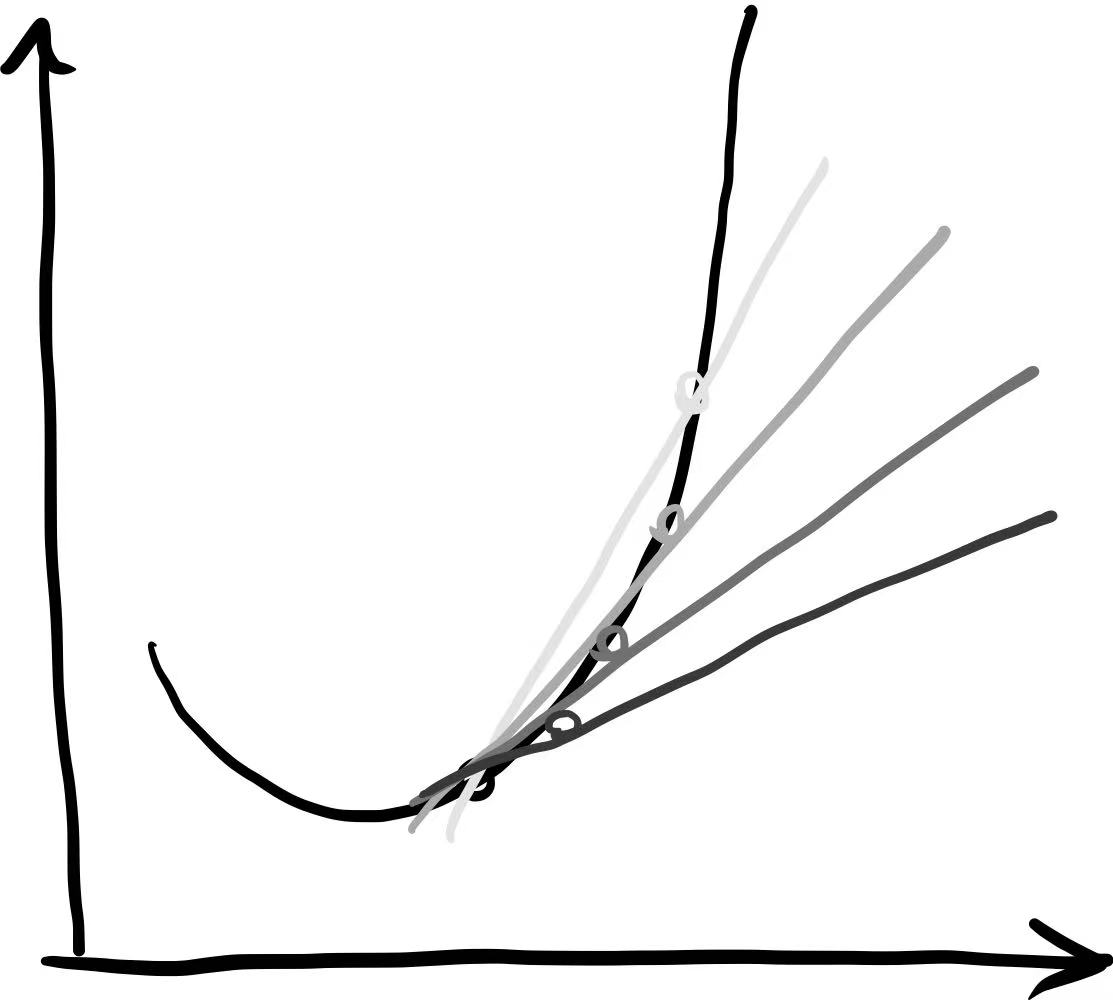
\includegraphics[width=0.9\textwidth]{img/image-20230614124234964.png}
\tcblower
\kaishu{\small 图像上, 不难看出, 当 $h$ 越来越小时, 两点的连线越来越趋向于切线, 当取到极限 $h\rightarrow0$ 时, 取到的这个值, 也就是导数, 便是切线的斜率.}
\end{tcolorbox}

物理教材更偏好

$\frac{\mathrm{d}y}{\mathrm{d}x}=\lim_{h\rightarrow0}\frac{f(x+h)-f(x)}{h}.$

\begin{newquote}
举一个例子, 若一个物体非匀速运动, 将速度 $v$ 表示为一个关于时间 $t$
的函数 $v(t)$, 那么便有加速度 (acceleration) 即速度的变化率:
$a(t)=v'(t)=\frac{\mathrm{d}v}{\mathrm{d}t}$.

另: 很多时候, 物理中, 关于时间的求导还有一个标记,
$\dot{f}\equiv \frac{\mathrm{d}f}{\mathrm{d}t}$\footnote{很多人经常吐槽物理中标记的不统一.
  个人当然也觉得, 如果有一套统一的标记, 信息的沟通自然会便利不少;
  但是学习的过程中, 既然标记不统一已经客观存在, 与其花时间吐槽,
  不如去抓住本质, 不要拘泥于标记, 而去理解标记背后的含义.}.
\end{newquote}

类似 $\frac{\mathrm{d}y}{\mathrm{d}x}$ 这样记法的好处是,
``变化率''这个概念被表现得很直观, 若有
$\frac{\mathrm{d}y}{\mathrm{d}x}=y'(x)$, 我们可以将它改写为
$\mathrm{d}y=y'(x)\mathrm{d}x$, 虽然``两边同乘 $\mathrm{d}x$''
这个说法非常不正确的, 但是从``变化率''的角度出发的确可以这么理解.

\begin{tcolorbox}[size=fbox, breakable, enhanced jigsaw, title={定理}]
若 $f(x)$ 在 $x=c$ 存在导数 (我们也可以说, 它在
$x=c$ 处可以被求导), 那么它在 $x=c$ 处连续.
\end{tcolorbox}

(不严格的) {\kaishu 证明}: 不使用 $\epsilon - \delta$ 语言的话,
只需证明 $\lim_{x\rightarrow c}f(x)=f(c)$ 即可. 于是, 对于有限的
$h$, $f(c+h)=f(c)+f(c+h)-f(c)=f(c)+\frac{f(c+h)-f(c)}{h}\cdot h$,
取极限 $h\rightarrow0$ 有
$\lim_{h\rightarrow0}f(c+h)=\lim_{h\rightarrow0}f(c)+\lim_{h\rightarrow0}\frac{f(c+h)-f(c)}{h}\cdot h=f(c)+f'(c)\cdot 0$,
第一个等号利用了极限的线性, 第二个等号则需要导数存在,
于是便有存在导数隐含 (imply) 连续.

若有函数 $f(x)$ 和 $g(x)$, 导数的一些性质:

\begin{itemize}

\item
  线性: $(af+bg)'(x)=af'(x)+bg'(x)$, 这里 $a$ 和 $b$ 是常数;
\item
  乘法法则 (product rule) : $(fg)'(x)=f'(x)g(x)+f(x)g'(x)$;
\item
  除法法则 (quotient rule) : $\left(\frac{f}{g}\right)'(x)=\frac{f'(x)g(x)-f(x)g'(x)}{g^2(x)}$,
  若 $g(x)\neq 0$.
\end{itemize}

第一条性质可以由极限的线性而来; 第二条和第三条可以分别令
$h(x)=f(x)g(x)$ 和 $h(x)=\frac{f(x)}{g(x)}$, 然后将 $h(x)$
代入导数的定义.

下面是一个非常 trivial 的例子,

\begin{newquote}
\textbf{例子}: $y(x)=x^2$, 求 $y'(x)$. 利用定义:

$\begin{aligned}y'(x)=&\lim_{h\rightarrow0}\frac{(x+h)^2-x^2}{h}\\=&\lim_{h\rightarrow0}\frac{x^2+h^2+2xh-x^2}{h}\\=&\lim_{h\rightarrow0}(2x+h^2)\\=&2x.\end{aligned}$
\end{newquote}

不难将结果推广为

$\boxed{\frac{\mathrm{d}}{\mathrm{d}x}x^n=nx^{n-1}}.$

\begin{newquote}
这样一来, 初中阶段得求二次函数在某点的切线就很 trivial 了. 例如: 求 $y (x)=ax^2+bx+c$, 在 $x=d$ 处的切线的表达式.

先对函数进行求导, $y'(x)=2ax+b$, 代入 $x=d$, 得到在 $x=d$ 处函数图像切线的斜率, $y'(c)=2ad+b$.

再将 $x=c$ 代入原函数, 得到, $y(c)=ad^2+bd+c$, 即切线的还经过 $(d, ad^2+bd+c)$ 这个点.

已知切线经过点 $(d, ad^2+bd+c)$, 且斜率为 $(2ad+b)$, 易得该切线的表达式.
\end{newquote}

\end{tcolorbox}